\documentclass[UTF8]{ctexart}
%\usepackage{ctex}
\usepackage{amsmath,amsthm,amsfonts,amssymb,bm}
%\usepackage{xfrac}
\usepackage{graphicx}
\usepackage{float}
\usepackage{geometry}
%\usepackage{subfigure}
\usepackage{booktabs}
\title{\zihao{1}高等数学 $\cdot$ 无穷级数}
\author{\tt 21305337 \it  Betelgeuxe}
\date{\kaishu\today}
\geometry{papersize={210mm,297mm}}
\geometry{left=2.9cm,right=2.9cm,top=3.2cm,bottom=2.7cm}
\usepackage{fancyhdr}
\pagestyle{fancy}
\fancyhf{}
\fancyhead[L]{\leftmark}
\fancyhead[R]{\tt 21305337 \it  Betelgeuxe\\\kaishu 仅供学习参考,勿作商业用途}
\fancyfoot[C]{\thepage}
\usepackage{hyperref}
\usepackage{multicol}

\usepackage{lipsum,lmodern}
\usepackage{tcolorbox}
\usepackage{listings}
    \tcbuselibrary{skins, breakable, theorems}

    \newcommand\stressbox{\tcboxmath[colframe=red,colback=yellow!50!white]}
    \newcommand\stressarea{\tcboxmath[colframe=yellow!50!white,colback=yellow!50!white]}
    \newcommand\stress{\tcboxmath[colframe=yellow!50!white,colback=yellow!50!white,left=0mm,right=0mm,top=0mm,bottom=0mm]}
    \tcbset{colback=white}

    \newenvironment{itemizer}{\begin{itemize}}{\end{itemize}}
    \tcolorboxenvironment{itemizer}{blanker,before skip=12pt,after skip=12pt,borderline west={3mm}{0pt}{red}}
    \newenvironment{itemizeg}{\begin{itemize}}{\end{itemize}}
    \tcolorboxenvironment{itemizeg}{blanker,before skip=12pt,after skip=12pt,borderline west={3mm}{0pt}{green!78!black}}
    \newenvironment{itemizeb}{\begin{itemize}}{\end{itemize}}
    \tcolorboxenvironment{itemizeb}{blanker,before skip=12pt,after skip=12pt,borderline west={3mm}{0pt}{blue}}
    
\begin{document}
\everymath{\displaystyle}
\pagenumbering{Roman}
\maketitle
\tableofcontents
\newpage
\pagenumbering{arabic}
\section{基本概念与记号}
\paragraph{通项}$a_n,n\in\mathbb{Z}$
\paragraph{(无穷)数列}$\{a_n\},n\in\mathbb{Z}$
\paragraph{(级数的)部分和}$S_n=\sum_{k=1}^na_k$
\paragraph{部分和序列}$\{S_n\}$
\paragraph{级数的和/常数项无穷级数}$S=\sum_{k=1}^\infty a_k$
\subsection{数项级数的敛散性}
\noindent $n\rightarrow\infty$ 时,若$\{S_n\}\rightarrow S$,则称级数$\sum_{k=1}^\infty a_k$\textbf{收敛},若$\{S_n\}$没有极限,则称级数$\sum_{k=1}^\infty a_k$\textbf{发散}.

\noindent\textbf{证明数列发散的一些方法}
\begin{itemizeg}
\item 证明不同的子数列有不同的极限
\item $a_n\not\rightarrow 0(n\rightarrow\infty)\Longrightarrow\sum_{k=1}^\infty a_k\text{发散}$
\end{itemizeg}

\noindent\textbf{证明数列收敛的一些方法}
\begin{itemizer}
\item $\varepsilon-N$定义
\item 单调有界
\item 夹逼定理
\item 利用重要极限的结论
\end{itemizer}

\begin{tcolorbox}[colframe=blue,title={\subsection{柯西收敛原理(柯西准则)}}]
\noindent $\{a_n\}$有极限$\Longleftrightarrow\forall \varepsilon>0,\exists N,{\rm st.}\forall n,m\geq N,|a_n-a_m|<\varepsilon$.
\tcblower
$\sum_{k=1}^\infty a_k\text{收敛}\Longleftrightarrow
\text{对}\forall\varepsilon>0,\exists N,{\rm st.}\text{对}\forall n\geq N,p\in\mathbb{Z}^+,\left|\sum_{k=n+1}^{n+p}a_k\right|<\varepsilon$.
\end{tcolorbox}

\subsection{收敛级数的性质}
\begin{itemizeb}
\item 若$\sum_{k=1}^\infty a_k=S_1,\ \sum_{k=1}^\infty b_k=S_2$,则$\sum_{k=1}^\infty(pa_k+qb_k)=pS_1+qS_2,\ p,q\in\mathbb{R}.$
\item 修改级数的有限项,级数的敛散性不变.
\item 给收敛级数的项任意加括号后,仍然收敛到原级数的和;给级数任意加括号后发散,则原级数发散.
\end{itemizeb}

\section{正项级数的收敛判别法}
\paragraph{正项级数}每项都非负的级数称为正项级数.
\paragraph{命题}正项级数$\sum_{n=1}^\infty n_k$收敛$\Longleftrightarrow\{S_n\}$有上界.


\begin{tcolorbox}[colframe=blue,sidebyside,title={\subsection{{\color{red}{[正项级数]}}比较判别法}}]
\noindent {\textbf{正项级数}$\sum_{n=1}^\infty u_n,\sum_{n=1}^\infty v_n$满足\stress{u_n\leq v_n} $(n=1,2,\cdots)$,则}
$$\stressarea{
    \begin{aligned}
        \sum_{n=1}^\infty u_n\text{发散}\Longrightarrow\sum_{n=1}^\infty v_n\text{发散},\\
        \sum_{n=1}^\infty v_n\text{收敛}\Longrightarrow\sum_{n=1}^\infty u_n\text{收敛}.
    \end{aligned}}$$
\tcblower
\noindent\textbf{极限形式}

\noindent \leftline{\textbf{正项级数}$\sum_{n=1}^\infty u_n,\sum_{n=1}^\infty v_n$满足}

{\stress{\lim_{n\rightarrow\infty}\frac{u_n}{v_n}=h},且$0<h<+\infty$\text{,则}}

$$\stressarea{\sum_{n=1}^\infty u_n\text{与}\sum_{n=1}^\infty v_n\text{敛散性相同}.}$$
\end{tcolorbox}

\begin{tcolorbox}[colframe=blue,title={\subsection{{\color{red}{[正项级数]}}比式判别法(达朗贝尔判别法)}}]
\noindent \textbf{正项级数}$\sum_{n=1}^\infty u_n$满足\stress{\lim_{n\rightarrow\infty}\frac{u_{n+1}}{u_n}=l},则

$$\stressarea{
    \begin{aligned}
        &\text{当}l<1,\text{级数收敛},\\
        &\text{当}l>1,\text{级数发散},\\
        &\text{当}l=1,\text{可能收敛也可能发散}.
    \end{aligned}}$$
    \begin{tcolorbox}[colframe=white!60!black,title={拉阿伯判别法*(针对$l=1$的情况)}]
        \noindent \textbf{正项级数}$\sum_{n=1}^\infty u_n(u_n\not=0)$满足\stress{\lim_{n\rightarrow\infty}n\left(\frac{u_n}{u_{n+1}}-1\right)=R},则
        
        $$\stressarea{
            \begin{aligned}
                &\text{当}R<1,\text{级数发散},\\
                &\text{当}1<R\leq+\infty,\text{级数收敛},\\
                &\text{当}R=1,\text{可能收敛也可能发散}.
            \end{aligned}}$$
    \end{tcolorbox}
        
\end{tcolorbox}

\begin{tcolorbox}[colframe=blue,title={\subsection{{\color{red}{[正项级数]}}根式判别法(柯西判别法)}}]
\noindent \textbf{正项级数}$\sum_{n=1}^\infty u_n$满足\stress{\lim_{n\rightarrow\infty}\sqrt[n]{u_n}=l},则

$$\stressarea{
    \begin{aligned}
        &\text{当}l<1,\text{级数收敛},\\
        &\text{当}l>1,\text{级数发散},\\
        &\text{当}l=1,\text{可能收敛也可能发散}.
    \end{aligned}}$$
\end{tcolorbox}

\begin{tcolorbox}[colframe=blue,title={\subsection{{\color{red}{[正项级数]}}柯西积分判别法}}]
    \begin{tcolorbox}[colframe=white!60!black,title={无穷积分}]
    \noindent 若极限$\lim_{A\rightarrow+\infty}\int_a^Af(x){\rm d}x$存在,则称无穷积分$\int_a^{+\infty}f(x){\rm d}x$收敛,并记

    $$\stressarea{\int_a^{+\infty}f(x){\rm d}x=\lim_{A\rightarrow+\infty}\int_a^Af(x){\rm d}x,}$$
    若$A\rightarrow+\infty$时$\int_a^Af(x){\rm d}x$没有极限,则称无穷积分$\int_a^{+\infty}f(x){\rm d}x$发散.
    \end{tcolorbox}
\textbf{正项级数}$\sum_{n=1}^\infty u_n(u_n\not=0)$,若$\exists f(x)>0,\stress{f(x)\searrow,{\rm st.}u_n=f(n),(n=1,2,\cdots)}$则

$$\stressarea{\sum_{n=1}^\infty u_n(u_n\not=0)\text{\quad 与\quad}\int_1^{+\infty}f(x){\rm d}x\text{\quad 敛散性相同}.}$$
\end{tcolorbox}

\newpage
\section{任意项级数}
\paragraph{交错级数}一项正、一项负交错排列的级数.

\begin{tcolorbox}[colframe=blue,title={\subsection{{\color{red}{[交错级数]}}莱布尼兹判别法}}]
\noindent 若\textbf{交错级数}$\sum_{n=1}^\infty(-1)^{n-1}u_n$或$\sum_{n=1}^\infty(-1)^{n}u_n$满足$\stress{u_n>0,u_{n+1}\leq u_n,\lim_{n\rightarrow\infty}u_n=0}$,则
$$\stressarea{\text{级数收敛,且}S\text{与}u_1\text{同号,}|S|<|u_1|.}$$
\end{tcolorbox}

\subsection{绝对收敛与条件收敛}
$$\stressbox{\sum_{n=1}^\infty |u_n|\text{收敛}\Longrightarrow\sum_{n=1}^\infty u_n\text{收敛}}$$
\paragraph{绝对收敛}若正项级数级数$\sum_{n=1}^\infty |u_n|$收敛,则称$\sum_{n=1}^\infty u_n$\textbf{绝对收敛}.
\paragraph{条件收敛}若级数$\sum_{n=1}^\infty u_n$收敛,但$\sum_{n=1}^\infty u_n$发散,则称$\sum_{n=1}^\infty u_n$\textbf{条件收敛}.

\begin{tcolorbox}[colframe=white!60!black,title={Tips}]
\noindent 可以利用“绝对收敛级数”和“比值判别法”证明:若$\stress{\lim_{n\rightarrow\infty}\left|\frac{u_{n+1}}{u_n}\right|=l}$,则

$$\stressarea{
    \begin{aligned}
        &\text{当}l<1,\text{级数收敛},\\
        &\text{当}l>1,\text{级数发散},\\
        &\text{当}l=1,\text{可能收敛也可能发散}.
    \end{aligned}}$$
\end{tcolorbox}

\paragraph{级数的重排}映射$f:\{1,2,\cdots\}\rightarrow\{1,2,\cdots\}称为级数的重排.$



\begin{itemizeg}
    \item []\!\!\!\!\!\!\!\! \textbf{绝对收敛级数的性质}\
    \item 绝对收敛级数$\sum_{n=1}^\infty u_n=\sum_{u_n>0}u_n+\sum_{u_n<0}u_n,$其中$\sum_{u_n>0}u_n=\sum_{n=1}^\infty \frac{|u_n|+u_n}{2}.$
    \item 收敛的正项级数(绝对收敛级数)重排后仍然收敛(绝对收敛)于原来的和,即绝对收敛级数满足\textbf{加法交换律}(无限项).
    \item\textbf{柯西定理\ } $\sum_{n=1}^\infty u_n$绝对收敛于$A,\sum_{n=1}^\infty v_n$绝对收敛于$B,$则$\sum_{n=1}^\infty u_nv_n$绝对收敛于$AB$,即绝对收敛的级数有乘法运算.
\end{itemizeg}

\subsection{阿贝尔判别法、狄利克雷判别法}

\begin{tcolorbox}[colframe=green!66!black,sidebyside,title=\bf{阿贝尔变换(离散型分部求和公式)、阿贝尔引理(阿贝尔不等式)}]
\noindent 设有数列$\{a_n\},\{b_n\}$,$B_n=\sum_{i=1}^ka_n$,则有
$$\stressarea{\sum_{i=1}^na_ib_i=\sum_{i=1}^{n-1}(a_i-a_{i-1})B_i+a_nB_n}$$
\tcblower
\noindent 设数列$\{a_n\}$是单调的,$B_n=\sum_{i=1}^ka_n$满足$|B_i|\leq M$,则有
$$\stressarea{\left|\sum_{i=1}^na_ib_i\right|\leq M(|a_1|+2|a_n|)}$$
\end{tcolorbox}

\begin{tcolorbox}[colframe=blue,title={\subsubsection{{\color{red}{[级数的积]}}狄利克雷判别法}}]
若$\stress{\lim_{n\rightarrow\infty}a_n=0,\text{数列}\{a_n\}\text{单调}}$;$\stress{\text{部分和数列}\left\{\sum_{i=1}^nb_i\right\}\text{有界}}$,则$\sum_{k=1}^\infty a_kb_k$收敛.
\tcblower
注:其中$\{a_n\}$不需要求和,实际上在证明过程中求了差分;而$\{b_n\}$需要求和.

使用狄利克雷判别法的关键是\underline{如何拆分成两个子数列的积}.

莱布尼兹判别法是狄利克雷判别法的特例.
\end{tcolorbox}

\begin{tcolorbox}[colframe=blue,title={\subsubsection{{\color{red}{[级数的积]}}阿贝尔判别法}}]
若$\stress{\text{数列}\{a_n\}\text{单调有界}};\stress{\text{级数}\sum_{i=1}^\infty b_i\text{收敛}}$,则$\sum_{k=1}^\infty a_kb_k$收敛.
\end{tcolorbox}

\begin{tcolorbox}[colframe=white!60!black,title={Tips}]
阿贝尔判别法相比狄利克雷判别法,$\{a_n\}$的条件更弱,$\{b_n\}$的条件更强.

狄利克雷判别法和阿贝尔判别法常用于判别条件收敛,判别绝对收敛有时用更弱的结论即可.
\end{tcolorbox}

\newpage

\section{函数项级数}
\subsection{基本概念与记号}
\subsubsection{函数项级数}

\paragraph{函数项级数}$\sum_{n=1}^\infty u_n(x)=u_1(x)+u_2(x)+\cdots+u_n(x)+\cdots$

\paragraph{收敛点(发散点)}若$\sum_{n=1}^\infty u_n(x_0)$收敛(发散),则称$x_0$为$\sum_{n=1}^\infty u_n(x)$的收敛点(发散点).

\paragraph{收敛域(发散域)}函数项级数的全体收敛点组成的集合,记作$X$.

\paragraph{和函数}$S(x)\equiv\sum_{n=1}^\infty u_n(x),\ x\in X.$

\subsubsection{函数序列}

\paragraph{函数序列}$\{f_n(x)|n=1,2,\cdots\}$

\paragraph{收敛点}若$\lim_{n\rightarrow\infty}f_n$存在,则称$\{f_n(x)\}$\textbf{在$x_0$点收敛},称$x_0$为$\{f_n(x)\}$的收敛点.

\paragraph{收敛域}函数序列的全体收敛点组成的集合,也记作$X$.

\paragraph{极限函数}$f(x)=\lim_{n\rightarrow\infty}f_n(x),\ \forall x\in X.$

\subsection{一致收敛的判定}

\begin{tcolorbox}[colframe=green!66!black,title=\subsubsection{序列的一致收敛}]
\paragraph{定义}若$f_n\rightarrow f(x),$对$\forall\varepsilon>0,\ \exists N(\stress{N\text{与}x\text{无关}},$可与$\varepsilon$有关$)$st.对$\forall x\in X,\ $当$n>N$时$|f_n(x)-f(x)|<\varepsilon$,则称$\{f_n(x)\}$在$X$上\textbf{一致收敛}于$f(x)$,

记作$\stress{f_n(x)\rightrightarrows f(x),\ x\in X\ (n\rightarrow\infty)}.$($\varepsilon-N$定义)

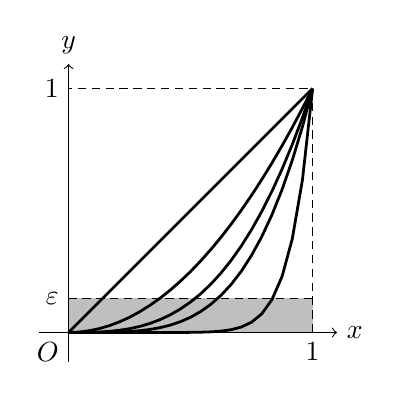
\begin{tikzpicture}[scale=3.1]
    \fill[white!75!black] (0,0)--(1,0)--(1,0.14)--(0,0.14);
    \draw[->](-0.12,0)--(0,0)node[below left]{$O$}--(1.1,0) node[right]{$x$};
    \draw[->](0,-0.12)--(0,1.1) node[above]{$y$};
    \draw[densely dashed] (1,0)node[below]{$1$}--(1,1)--(0,1)node[left]{$1$};
    \draw[densely dashed] (0,0.14)node[left]{$\varepsilon$}--(1,0.14);
    \draw [color=black,line width=1pt,domain=0:1] plot (\x,\x);
    \draw [color=black,line width=1pt,domain=0:1] plot (\x,\x^2);
    \draw [color=black,line width=1pt,domain=0:1] plot (\x,\x^3);
    \draw [color=black,line width=1pt,domain=0:1] plot (\x,\x^4);
    \draw [color=black,line width=1pt,domain=0:1] plot (\x,\x^11);
\end{tikzpicture}
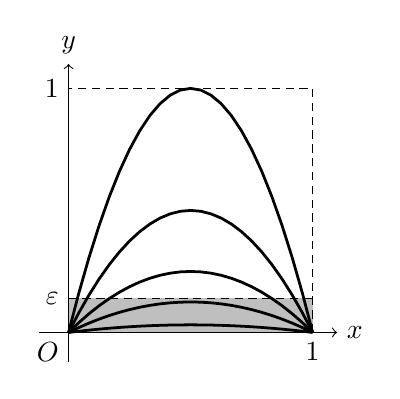
\begin{tikzpicture}[scale=3.1]
    \fill[white!75!black] (0,0)--(1,0)--(1,0.14)--(0,0.14);
    \draw[->](-0.12,0)--(0,0)node[below left]{$O$}--(1.1,0) node[right]{$x$};
    \draw[->](0,-0.12)--(0,1.1) node[above]{$y$};
    \draw[densely dashed] (1,0)node[below]{$1$}--(1,1)--(0,1)node[left]{$1$};
    \draw[densely dashed] (0,0.14)node[left]{$\varepsilon$}--(1,0.14);
    \draw [color=black,line width=1pt,domain=0:1] plot (\x,{4*\x*(1-\x)});
    \draw [color=black,line width=1pt,domain=0:1] plot (\x,{2*\x*(1-\x)});
    \draw [color=black,line width=1pt,domain=0:1] plot (\x,{1*\x*(1-\x)});
    \draw [color=black,line width=1pt,domain=0:1] plot (\x,{1/2*\x*(1-\x)});
    \draw [color=black,line width=1pt,domain=0:1] plot (\x,{1/8*\x*(1-\x)});
\end{tikzpicture}
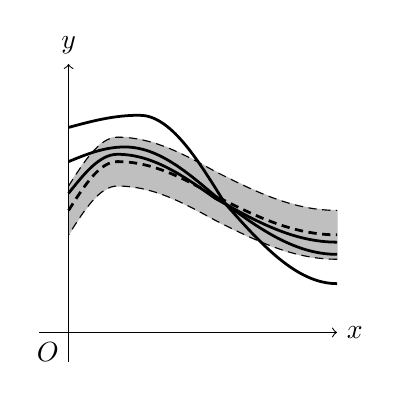
\begin{tikzpicture}[scale=3.1]
    \filldraw[white!75!black] (0,.6)sin(.2,.8)cos(.6,.66)sin(1.1,.5)
        --(1.1,.3)cos(.6,.46)sin(.2,.6)cos(0,.4);
    \draw[->](-0.12,0)--(0,0)node[below left]{$O$}--(1.1,0) node[right]{$x$};
    \draw[->](0,-0.12)--(0,1.1) node[above]{$y$};
    \draw[densely dashed] (1.1,.3)cos(.6,.46)sin(.2,.6)cos(0,.4);
    \draw[densely dashed] (0,.6)sin(.2,.8)cos(.6,.66)sin(1.1,.5);
    \draw[color=black,densely dashed,line width=1pt,domain=0:1] (0,.5)sin(.2,.7)cos(.6,.56)sin(1.1,.4);
    \draw [color=black,line width=1pt,domain=0:1] (0,.84)sin(.29,.89)cos(.64,.53)sin(1.1,.2);
    \draw [color=black,line width=1pt,domain=0:1] (0,.7)sin(.23,.76)cos(.6,.56)sin(1.1,.32);
    \draw [color=black,line width=1pt,domain=0:1] (0,.57)sin(.2,.73)cos(.6,.55)sin(1.1,.37);
\end{tikzpicture}
\end{tcolorbox}


\begin{itemizeg}
    \item[]\textbf{可证明序列一致收敛的两个命题}
    \item 设$\{f_n(x)\}$在$X$上收敛到$f(x)$,若$\exists$数列$\{a_n\},a_n\rightarrow0(n\rightarrow\infty)$\ st.
    $$|f_n(x)-f(x)|\leq a_n,\ x\in X,\ n>N,$$
    则$f_n(x)\rightrightarrows f(x),\ x\in X\ (n\rightarrow\infty).$(P241命题1)
    \item $\sum_{n=1}^\infty u_n(x)$在$X$上一致收敛$\Longrightarrow u_n(x)\rightrightarrows 0,\ x\in X\ (n\rightarrow\infty).$(P243定理1)
\end{itemizeg}

\begin{itemizeb}
    \item[]\textbf{可证明序列不一致收敛的两个命题}
    \item 设$\{f_n(x)\}$在$X$上收敛到$f(x)$,若$\exists\{x_n\}\ (x_n\in X)\ $st.当$n>N$时,
    $$|f_n(x_n)-f(x_n)|\geq l,\quad l>0\text{为常数}$$
    $$\text{或}\quad |f_n(x_n)-f(x_n)|\rightarrow k\neq 0,\quad k\text{为常数}$$
    则$\{f_n(x)\}$在$X$上不一致收敛.(P242命题1,2)

    Tips:通常使$x_n\rightarrow x_d$的速度非常快,其中$x_d\not\in X$.
    \item$ u_n(x)$在$X$上不一致收敛于0\ $\Longrightarrow\sum_{n=1}^\infty u_n(x)$在$X$上不一致收敛.(P243定理1之逆否命题)
\end{itemizeb}

\begin{tcolorbox}[colframe=green!66!black,title=\subsubsection{函数项级数的一致收敛}]
    \paragraph{定义}设函数项级数$\sum_{k=1}^\infty u_k(x)$中的每一项在$X$中有定义,若部分和数列$S_n=\sum_{k=1}^n u_k(x)$在集合$X$上一致收敛,则称级数$\sum_{k=1}^\infty u_k(x)$在$X$上\textbf{一致收敛}.

\tcblower

    \subsubsection{一致收敛的柯西准则}
    $\sum_{k=1}^\infty u_k(x)$在$X$上一致收敛$\Longleftrightarrow$
        
    \qquad 对$\forall\varepsilon>0,\exists N=N(\varepsilon),$st.对$\forall p\in\mathbb{Z}^+,\left|\sum_{k=n+1}^{n+p}u_n(x)\right|<\varepsilon$对$\forall x\in X$成立.
    \begin{tcolorbox}[colframe=blue,title={\subsubsection{{\color{red}{[函数项级数]}}强级数判别法}}]
        若$|u_n(x)|\leq a_n,\ \forall x\in X,\ n=1,2,\cdots,$且$\sum_{k=1}^\infty a_k$收敛\ $\Longrightarrow\sum_{k=1}^\infty u_k(x)$在$X$上\textbf{一致收敛}(且绝对收敛),并称$\sum_{k=1}^\infty a_k$为$\sum_{k=1}^\infty u_k(x)$的强级数.
    \end{tcolorbox}
\end{tcolorbox}

\begin{tcolorbox}[colframe=green!66!black,title=\subsubsection{一致有界}]
    \paragraph{定义}设$\{f_n(x)\}$在集合$X$上有定义,若$\exists$常数$M$,st.$\forall n\in\mathbb{Z}^+,\forall x\in X$,都有$|f_n(x)|\leq M,$则称$\{f_n(x)\}$一致有界.
\end{tcolorbox}

\begin{multicols}{2}
    \begin{tcolorbox}[colframe=blue,title={\subsubsection{{\color{red}{{\zihao{-5}[函数项级数的积]}}}狄利克雷判别法}}]
        若$(1)$对$\forall x\in X,\ \{a_n(x)\}$\textbf{对$n$单调},且$a_n(x)$\textbf{一致收敛于0}$(x\in X)$,
        
        $\quad\ (2)$部分和序列$\left\{\sum_{k=1}^nb_k(x)\right\}$在$X$上
        \textbf{一致有界},
        
        则$\sum_{k=1}^\infty a_k(x)b_k(x)$在$X$上\textbf{一致收敛}.
    \end{tcolorbox}
        
    \begin{tcolorbox}[colframe=blue,title={\subsubsection{{\color{red}{{\zihao{-5}[函数项级数的积]}}}阿贝尔判别法}}]
        若$(1)$对$\forall x\in X,\ \{a_n(x)\}$\textbf{对$n$单调}且在$X$上 \textbf{一致有界},
        
        $\quad\ (2)$级数$\sum_{k=1}^\infty b_k(x)$在$X$上\textbf{一致收敛},
        
        则$\sum_{k=1}^\infty a_k(x)b_k(x)$在$X$上\textbf{一致收敛}.
    \end{tcolorbox}
\end{multicols}

\subsection{一致收敛的性质}

\begin{tcolorbox}[colframe=green!66!black]
\subsubsection{和函数的连续性(求和与求极限可交换顺序)}

在闭区间$[a,b]$上,
$$\stress{\begin{cases}
    \text{每一项}u_n\text{都连续}\\
    \sum_{n=1}^\infty u_n(x)\text{一致收敛}
\end{cases}
\Longrightarrow
\begin{cases}
    S(x)=\sum_{n=1}^\infty u_n(x)\text{连续}\\
    {\color{blue}\lim_{x\rightarrow x_0}\sum_{n=1}^\infty}u_n(x)={\color{blue}\sum_{n=1}^\infty\lim_{x\rightarrow x_0}}u_n(x)
\end{cases}}$$

\subsubsection{逐项求积(求和与积分可交换顺序)}

    在闭区间$[a,b]$上,
    $$\stress{\begin{cases}
        \text{每一项}u_n\text{都可积}\\
        \sum_{n=1}^\infty u_n(x)\text{一致收敛}
    \end{cases}
    \Longrightarrow
    \begin{cases}
        S(x)=\sum_{n=1}^\infty u_n(x)\text{可积}\\
        {\color{blue}\int_a^b\sum_{n=1}^\infty}u_n(x){\rm d}x={\color{blue}\sum_{n=1}^\infty\int_a^b}u_n(x){\rm d}x
    \end{cases}}$$

\subsubsection{逐项求导(求和与求导可交换顺序)}

    在闭区间$[a,b]$上,
    $$\stress{\begin{cases}
        \text{每一项导函数}u'_n\text{都连续}\\
        \sum_{n=1}^\infty u_n(x)\text{点点收敛}\\
        \sum_{n=1}^\infty u'_n(x)\text{一致收敛}
    \end{cases}
    \Longrightarrow
    \begin{cases}
        S(x)=\sum_{n=1}^\infty u_n(x)\text{可导}\\
        {\color{blue}\left[\sum_{n=1}^\infty{\color{black}u_n(x)}\right]'}={\color{blue}\sum_{n=1}^\infty}u_n{\color{blue}'}(x)
    \end{cases}}$$
\end{tcolorbox}

\section{幂级数}
$$\sum_{n=0}^\infty a_n(x-x_0)^n=a_0+a_1(x-x_0)+a_2(x-x_0)^2+\cdots$$
\subsection{收敛半径}
\noindent$\sum_{n=0}^\infty a_n(x-x_0)^n$的收敛域有三种情况:

1)一个点$\{x_0\}$;\quad 2)以$x_0$为中心的区间,可能是开区间、闭区间、半开半闭区间;\quad 3)$\mathbb{R}$.

\begin{tcolorbox}[colframe=green!66!black,title=\subsubsection{阿贝尔定理}]
若$\sum_{n=0}^\infty a_nx^n$在点$x_1$收敛,则对$\forall x<|x_1|${\bf 绝对收敛}.

若$\sum_{n=0}^\infty a_nx^n$在点$x_2$发散,则对$\forall x>|x_2|$发散.
\end{tcolorbox}

\begin{multicols}{2}
    \begin{tcolorbox}[colframe=blue,title=\subsubsection{比式求$R$法}]
        若$\stress{\lim_{n\rightarrow\infty}\left|\frac{a_{n+1}}{a_n}\right|=l}$,则$\sum_{n=0}^\infty a_nx^n$的收敛半径$R$满足:
        $${R=\begin{cases}
            \stress{\frac{1}{l}},&0<l<+\infty,\\
            \ 0,&l=+\infty,\\
            +\infty,&l=0.
        \end{cases}}$$
    \end{tcolorbox}
        
    \begin{tcolorbox}[colframe=blue,title=\subsubsection{根式求$R$法}]
        若$\stress{\lim_{n\rightarrow\infty}\sqrt[n]{a_n}=l}$,则$\sum_{n=0}^\infty a_nx^n$的收敛半径$R$满足:
        $${R=\begin{cases}
            \stress{\frac{1}{l}},&0<l<+\infty,\\
            \ 0,&l=+\infty,\\
            +\infty,&l=0.
        \end{cases}}$$
    \end{tcolorbox}
\end{multicols}

\subsection{幂级数的性质}

\subsubsection{四则运算}
\begin{tcolorbox}[colframe=green!66!black]
在$\sum_{n=0}^\infty a_nx^n$与$\sum_{n=0}^\infty b_nx^n$都收敛的\textbf{开区域}内,有
$$\stress{\sum_{n=0}^\infty a_nx^n\pm\sum_{n=0}^\infty b_nx^n=\sum_{n=0}^\infty (a_n\pm b_n)x^n}$$
$$\left(\sum_{n=0}^\infty a_nx^n\right)\left(\sum_{n=0}^\infty b_nx^n\right)=\sum_{n=0}^\infty\ \sum_{i+j=n} a_ib_jx^n$$
\end{tcolorbox}

\subsubsection{内闭一致性} 
\begin{tcolorbox}[colframe=green!66!black]
设幂级数 $\sum_{n=0}^{\infty} a_{n} x^{n}$ 的收敛半径为 $R>0$, 则

(1)$\stress{\text{对}\forall\text{正数}b<R,\sum_{n=0}^{\infty} a_{n} x^{n}\text{在}[-b, b]\text{上一致收敛};}$

(2)若$\sum_{n=0}^{\infty} a_{n} x^{n}$在$x=R$收敛, 则它在$[0, R]$上一致收敛;

(3)若$\sum_{n=0}^{\infty} a_{n} x^{n}$在$x=-R$收敛,则它在$[-R, 0]$ 上一致收敛.
\end{tcolorbox}

\subsubsection{连续性、可积性、可微性(前一节的推论)}
\begin{tcolorbox}[colframe=green!66!black]
\paragraph{连续性}幂级数$\sum_{n=0}^{\infty}a_{n}x^{n}$的和函数 $S(x)$ 在其收敛区间$(-R, R)$ 内连续.

又若幂级数 $\sum_{n=0}^{\infty} a_{n} x^{n}$ 在 $x=R$ (或 $x=-R$ )处收敛,则 $S(x)$ 在 $x=R$ (或 $x=-R)$ 点处左(右)连续.
\tcbline
\paragraph{可积性}幂级数 $\sum_{n=0}^{\infty} a_{n} x^{n}$ 的和函数$S(x)$ 在收敛区间 $(-R, R)$ 内任一闭 区间上可积,且可逐项求积分,且逐项积分所得的新幂级数$\sum_{n=0}^{\infty} \frac{a_{n}}{n+1} x^{n+1}$的收敛半径$R_{1}=R$.
\tcbline
\paragraph{可微性}幂级数 $\sum_{n=0}^{\infty} a_{n} x^{n}$ 的和函数$S(x)$ 在其收敛区间 $(-R, R)$ 内可导,且可逐项求导,且逐项求导所得的新幂级数$\sum_{n=1}^{\infty}na_{n} x^{n-1}$ 的收敛 半径 $R_{2}=R$.

\qquad 更进一步,幂级数$\sum_{n=0}^{\infty} a_{n} x^{n}$ 的和函数 $S(x)$ 在收敛区间 $(-R, R)$内任意阶可导,且可逐项求任意阶导数,它们的收敛半径都是$R$.
\end{tcolorbox}

\newpage
\section{泰勒级数}
\subsection{部分基本定义与定理}
\begin{tcolorbox}[colframe=green!66!black]
\noindent 设$y=f(x)$在$x_0$处有任意阶导数,则级数
$\sum_{n=0}^{\infty} \frac{f^{(n)}\left(x_{0}\right)}{n !}\left(x-x_{0}\right)^{n} $称为 $f(x)$ 的\textbf{泰勒级数},记作
$$
f(x)\sim\sum_{n=0}^{\infty} \frac{f^{(n)}\left(x_{0}\right)}{n !}\left(x-x_{0}\right)^{n} .
$$
若一个函数的泰勒级数收敛到这个函数,称其泰勒级数为其\textbf{泰勒展开式}.
\tcbline
当$x_{0}=0$时$,\sum_{n=0}^{\infty} \frac{f^{(n)}(0)}{n !} x^{n}$称为$f(x)$的\textbf{麦克劳林级数}.
\tcbline
\paragraph{定理}幂级数展开式具有唯一性.
\paragraph{定理}设函数 $f(x)$ 在含有点 $x_{0}$ 的某个区间 $(a, b)$ 内有任意阶的导函数,则当$x\in(a,b),$
$$\stressbox{f(x)\text{能展开为泰勒级数}\Longleftrightarrow\lim_{n\rightarrow\infty}R_n(x)=0}$$

其中 $R_{n}(x)$ 为 $f(x)$ 的泰勒公式的余项,可表示成
$$R_{n}(x)=\frac{1}{(n+1) !} f^{(n+1)}\Big(x_{0}+\theta\left(x-x_{0}\right)\Big)\left(x-x_{0}\right)^{n+1},\quad 0<\theta<1,$$
$$\!\!\!\!\!\!\!\!\!\!\text{或}\quad R_{n}(x)=\frac{1}{(n+1) !} f^{(n+1)}(\xi)\left(x-x_{0}\right)^{n+1},\quad x_0<\xi<x\text{\ 或\ }x<\xi<x_0.$$
\end{tcolorbox}

\begin{tcolorbox}[colframe=blue,title=\subsection{求展开式的步骤}]
\paragraph{Step 1}求导,写出泰勒级数(展开式);

\paragraph{Step 2}利用幂级数的性质(可用“比式求$R$法”“根式求$R$法”)求出收敛半径,并进一步求出收敛域.

\paragraph{Step 3}在收敛域上讨论$R_n(x)\rightarrow0$何时成立,得出展开式成立的区间.
\end{tcolorbox}

\newpage
\subsection{一些常用的初等函数的泰勒展开式}
$$\begin{aligned}
\frac{1}{1-x}&=1+x+x^2+\cdots+x^n+\cdots&(-1<x<1)\\
e^{x}&=1+x+\frac{1}{2 !} x^{2}+\cdots+\frac{1}{n !} x^{n}+\cdots \hspace{3.5cm}&(-\infty<x<+\infty)\\
\sin x&=x-\frac{x^{3}}{3 !}+\frac{x^{5}}{5 !}+\cdots+(-1)^{n-1} \frac{x^{2 n-1}}{(2 n-1) !}+\cdots \hspace{2cm}&(-\infty<x<+\infty)\\
\cos x&=1-\frac{x^{2}}{2 !}+\frac{x^{4}}{4 !}+\cdots+(-1)^{n} \frac{x^{2 n}}{(2 n) !}+\cdots\hspace{3cm}&(-\infty<x<+\infty)\\
\arctan x&=x-\frac{x^{3}}{3}+\frac{x^{5}}{5}+\cdots+(-1)^{n} \frac{1}{2 n+1} x^{2 n+1}+\cdots\hspace{2cm}&(-1 \leqslant x \leqslant 1)\\
\ln (1+x)&=x-\frac{x^{2}}{2}+\frac{x^{3}}{3}+\cdots+(-1)^{n-1} \frac{x^{n}}{n}+\cdots\hspace{3cm}&(-1<x \leqslant 1)\\
(1+x)^{\alpha}&=1+\alpha x+\frac{\alpha(\alpha-1)}{2 !} x^{2}+\cdots+\frac{\alpha(\alpha-1) \cdots(\alpha-n+1)}{n !} x^{n}+\cdots&(-1<x<1)
\end{aligned}$$

\end{document}